\documentclass[10pt]{article}
\usepackage{setspace}
\usepackage{url}
\usepackage{graphicx}
\usepackage{geometry}
\geometry{letterpaper}
\begin{document}
\title{\vfill coffee\_shop: Investigations into modern word processors.}
\author{
Nathaniel Welch, Dr. Clark Turner\vspace{10pt} \\
California State Polytechnic University\vspace{10pt} \\
}
\date{\today}
\maketitle

\doublespacing

\vfill
\begin{abstract}
My senior project was spent building a desktop application similar to WriteRoom and OmmWriter. These two applications are both word processors for the Macintosh OS X operating system. Both of these applications are designed to be a reset on word processing software, bringing their interfaces back to the days of Microsoft Word 3.0 and Word Perfect. They do this by spending more time on focusing on the design of the software interface, and focusing on keeping it minimalistic, instead of filling the product with new obscure features, which is a common complaint against the current iterations of Microsoft Word.

The final application, named coffee\_shop, ended up not meeting my expectations. Having spent most of my education developing applications for the internet, instead of the desktop, I ran into pitfalls which, if this had been an internet application, wouldn't have been problematic.
\end{abstract}

% Table of Contents
\thispagestyle{empty}
\newpage
\singlespacing
\thispagestyle{empty}
\tableofcontents
\newpage
\doublespacing

\section{Introduction}

Depending on the job, people use different tools. Some tools are incredibly specialised, such as post hole diggers and PVC pipe warmers. Others are much more generic, such as hammers and cameras. Notice though, that in the hardware world, the majority of tools serve one job. That job, such as hammering, can be applied to a wide variety of ways (hammering in a nail, breaking apart structures, putting stakes in the ground). In the software world, historically tools have been built to be much more generic. Microsoft Word for example not only let you write documents, but also create spreadsheets, resumes and many other things. While this has let Microsoft make more money by selling their software to a wider variety of needs, it has created software that is hard to use and hard to maintain. To fight this, companies and individuals are starting to create software that have less features and are easier to use.

\section{Problem description}

The problem coffee\_shop tries to tackle is whether or not developing a desktop application focused on writing, instead of formating, is a good idea.

\section{Survey of relevant work}

Before starting the project, I surveyed a variety of word processor programs and interviewed individuals about their writing habits. The survey I distributed was simple and open-ended. I asked users what types of documents they wrote, what they disliked about their current word processor and what they liked and wanted in their word processor.

I discovered that there were two groups of users of word processors in my survey group. There were those who wrote in a corporate or academic environment and those that wrote for themselves. The users that wrote more for academia and corporate positions tended to want lots of formatting options. Users writing for themselves usually wanted something that hid everything and let them just write.

Every single one of my responders despised Microsoft Word's auto-correct but still wanted spell check.

I decided to name my user group Johnny, based on two different people that I interviewed and the responses from my survey. Johnny writes fiction in his free time and aspires to be a writer. He is currently employed doing other things, so he uses his word processor as he commutes and during his time off. Most of what Johnny writes tends to be one or two pages, but he has been known to turn out novels depending on his mood.

\subsection{Professional Offerings}

As stated earlier, there are a variety of choices in the word processor market. The ones I tried and examined were chosen both by their reputation and based on how easily I could get my hands on a copy.

\subsubsection{Microsoft Word 2010}

Microsoft Word 2010 is a pretty expansive program. It easily has more features and options than any of the other products I tested.

\begin{figure}
   \centering
      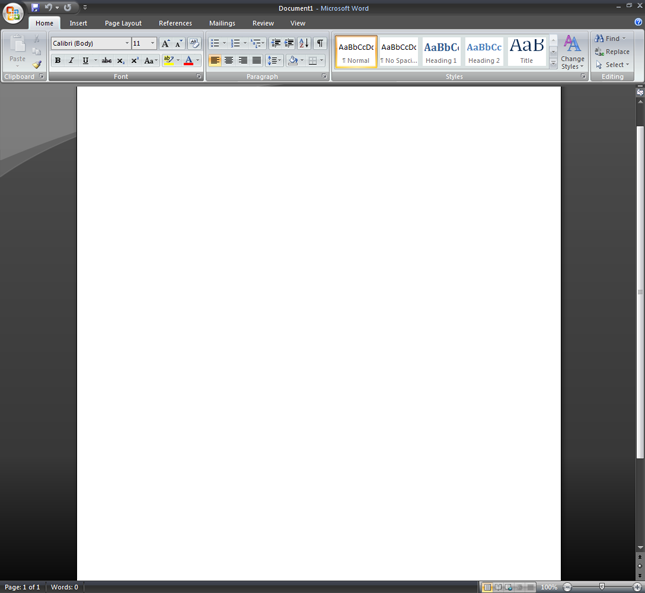
\includegraphics[width=130mm]{images/BlankWord.png}
   \caption{Microsoft Word 2010 with no text.}
\end{figure}

Its while it has a relatively easy to interpret selection of main controls on the top of the page, most options are hidden under a variety of menus. Disabling features that many who I surveyed complained about, such as auto-correct, took a few minutes to find the right check box.

\begin{figure}
   \centering
      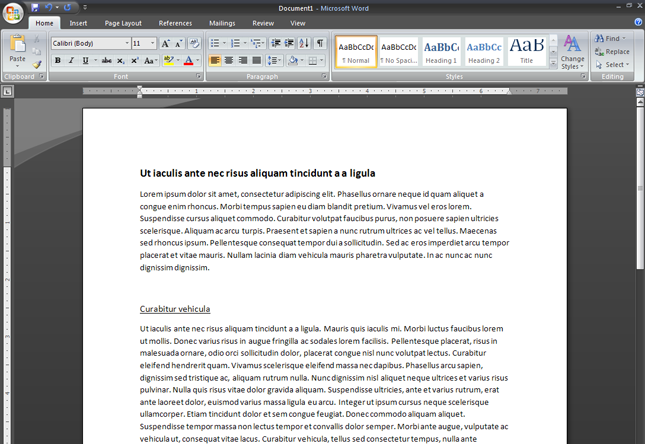
\includegraphics[width=130mm]{images/TextWord.png}
   \caption{Microsoft Word 2010 with text.}
\end{figure}

Despite its weight, Word is incredibly powerful, and no matter what a user needs to do, Word should be able to do it.

\subsubsection{Microsoft Word 5.5}

Originally released in 1991\cite{infoworld}, Microsoft Word 5.5 is an interesting beast. 5.5's initial downside is that it needs to be run in DosBox. The cool thing about DosBox though, is that it means I can run 5.5 on Linux and on just about every other machine that it supports. But 5.5 comes from before the days where everything is just one executable. The user install experience is incredibly slow and time consuming. 5.5 extracts four hundred files before setup, and then another two hundred during the install process.

\begin{figure}
   \centering
      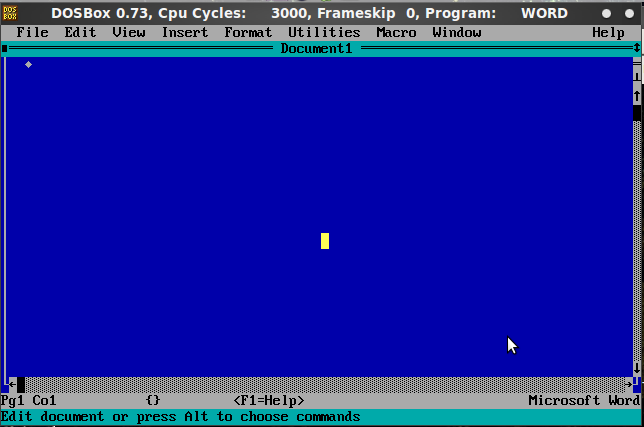
\includegraphics[width=130mm]{images/w55_1.png}
   \caption{Microsoft Word 5.5.}
\end{figure}

Once you are inside 5.5, the experience is relatively nice. Document navigation was done entirely via the keyboard. It reminded me a lot of Pico, and was a joy to use. The user can also select text with the mouse, and we can see how the experience in 5.5 turned into that of Microsoft Word 2010.

5.5 offered no color or font customizations, although the user could go full screen, which was very nice. Page breaks were implied with an emphasized dotted line.

\subsubsection{Pages}

The Apple offering in the word processor space. I found Pages rather nice to use, and its full screen mode was very similar to what I was looking to make. The downsides were simple though. Pages default file type cannot be read by any other program, and you could do very little to customize the user interface.

\subsubsection{OpenOffice}

OpenOffice Writer 3 seems to be on-par with current Microsoft Word offerings. The product has a ton of features, most of which were hidden behind obscure icons and menus.

\begin{figure}
   \centering
      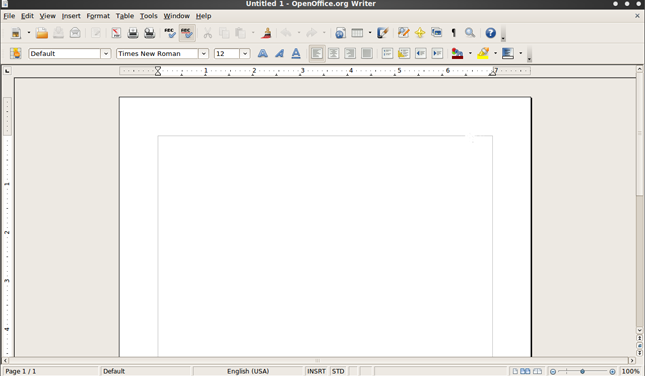
\includegraphics[width=130mm]{images/oo1.png}
   \caption{...}
\end{figure}

Writer was nice in that it always opens a new empty document so you can start writing immediately.

\begin{figure}
   \centering
      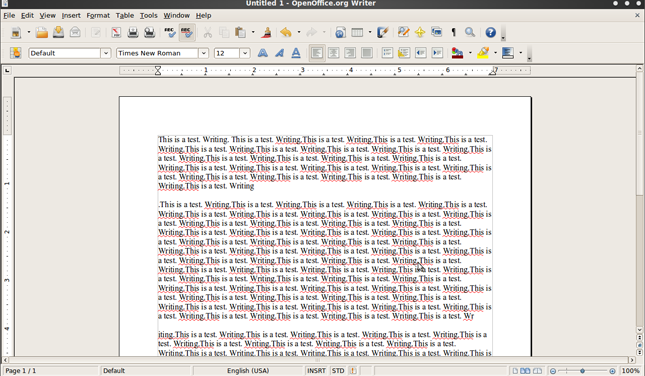
\includegraphics[width=130mm]{images/oo2.png}
   \caption{...}
\end{figure}

The full screen mode looked nice, but tended to crash when transitioning in and out.

Writer also had an easy to use ``export to PDF'' feature. Spell check was also easy to find compared to many of the other programs examined.

\begin{figure}
   \centering
      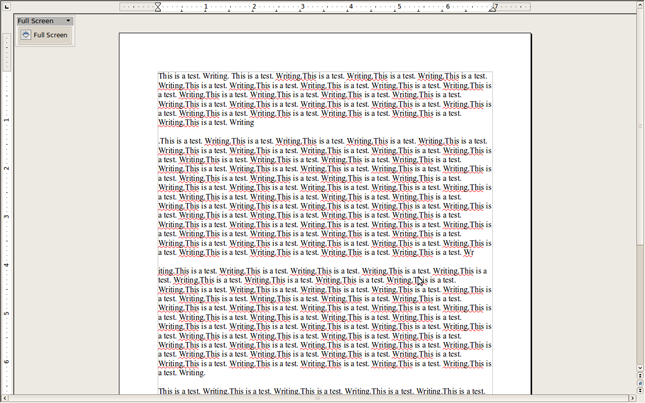
\includegraphics[width=130mm]{images/oo3.png}
   \caption{...}
\end{figure}

You could customize a lot of things in Writer, but it was annoying that you had to select all of the text to change the document color scheme. In contrast though, Writer supported more fonts than any of the other programs.

Overall Writer is a nice offering considering it is free, but the interface can be intimidating, especially if you have no idea what all of the buttons do.

\subsubsection{Vim}

According to the Vim website, vim.org, ``Vim is a highly configurable text editor built to enable efficient text editing. It is an improved version of the vi editor distributed with most UNIX systems'' \cite{vimabout}. I love Vim, and since starting this project, I've pretty much decided that in almost every scenario, I would use Vim to write things.

\begin{figure}
   \centering
      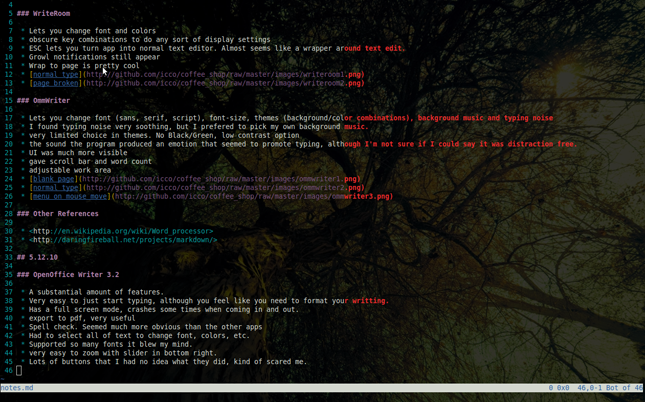
\includegraphics[width=130mm]{images/vim2.png}
   \caption{...}
\end{figure}

I currently am using Vim to write this paper, I used it to write almost all of the code for coffee\_shop and I have been using it pretty exclusively for the last four years.

\begin{figure}
   \centering
      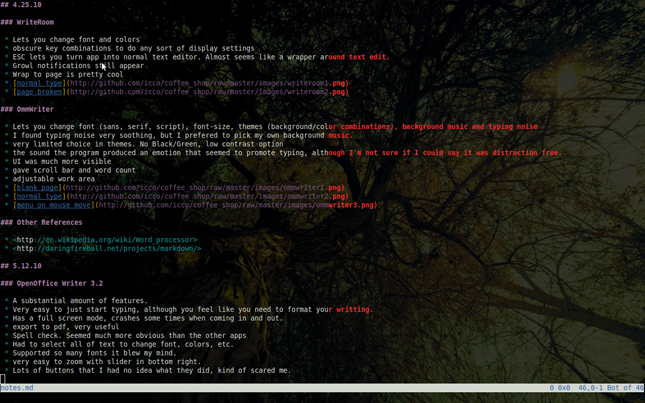
\includegraphics[width=130mm]{images/vim3.png}
   \caption{...}
\end{figure}

Vim has its issues though. It has a really difficult learning curve. In fact, without working for a company where almost every developer used it, I probably would have given up long ago. Most people give up quickly because they do not understand why Vim tries to make sure you never use the mouse. In their defense, this is fair, the user interface does not tell the user much at all, and expects the user to know all of the magic incantations to get things to happen. I have heard that emacs is the same way, but I have never used it.

\subsection{Similar implementations}

These are programs I am trying to emulate.

\subsubsection{WriteRoom}

WriteRoom is a piece of software for OS X by HogBay Software \cite{writeroom}. By default WriteRoom opens in full screen. Pressing escape though turns the app into a normal windowed text editor. This windowed text editor looks very similar to OS X's Text Edit.

\begin{figure}
   \centering
      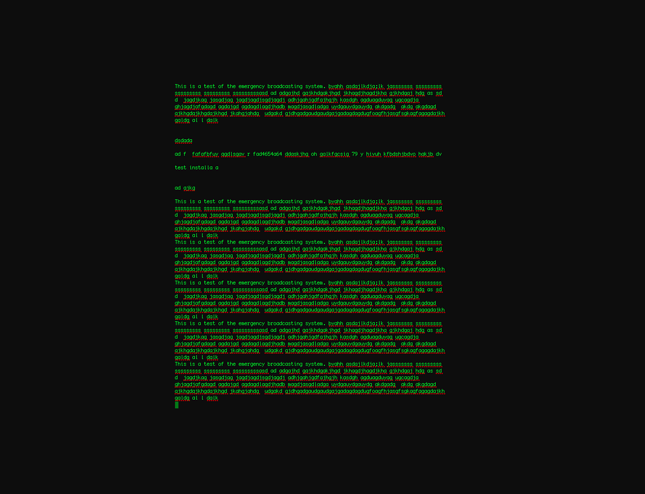
\includegraphics[width=130mm]{images/writeroom1.png}
   \caption{...}
\end{figure}

WriteRoom has a lot of cool customizations. It lets the user choose colors and fonts. It also does a really nice job wrapping and splitting up pages.

\begin{figure}
   \centering
      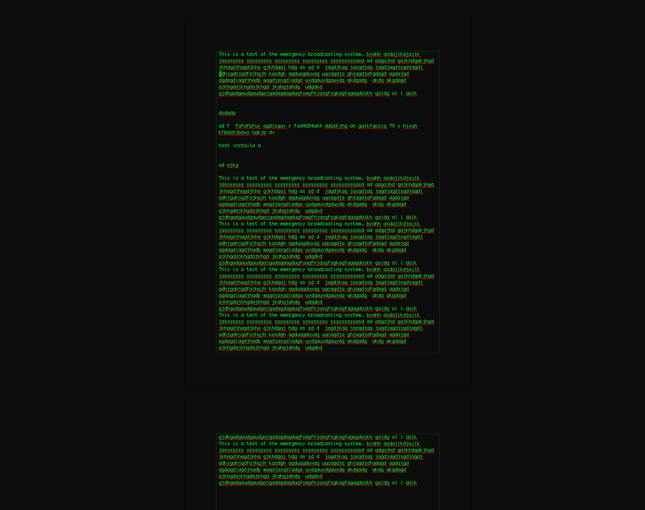
\includegraphics[width=130mm]{images/writeroom2.png}
   \caption{...}
\end{figure}

The only thing I found annoying was that you needed to know obscure key combinations to do change any sort of display settings. This seemed weird, because while key bindings let you keep the interface simple, users can't use them if they aren't taught them when the application opens.

\subsubsection{OmmWriter}

OmmWriter \cite{ommwriter} is similar to WriteRoom in its feature set, except that it focuses around themes. Users select from a limited set of fonts, background and color combinations, background music, and typing noises.

\begin{figure}
   \centering
      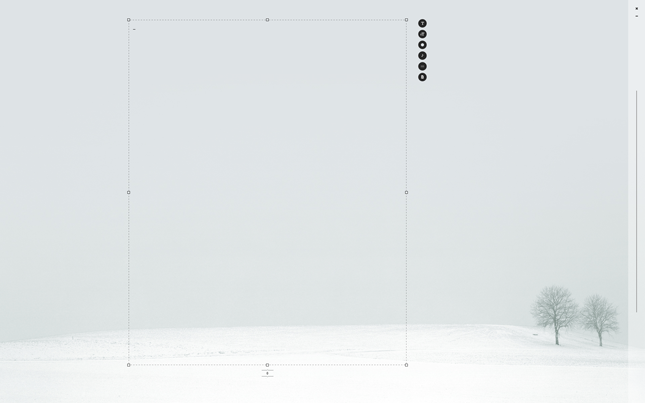
\includegraphics[width=130mm]{images/ommwriter1.png}
   \caption{...}
\end{figure}

The typing noise was quite an interesting idea. I tended to mute the background music, but noise of clicking typewriter keys ended up being quite soothing.

\begin{figure}
   \centering
      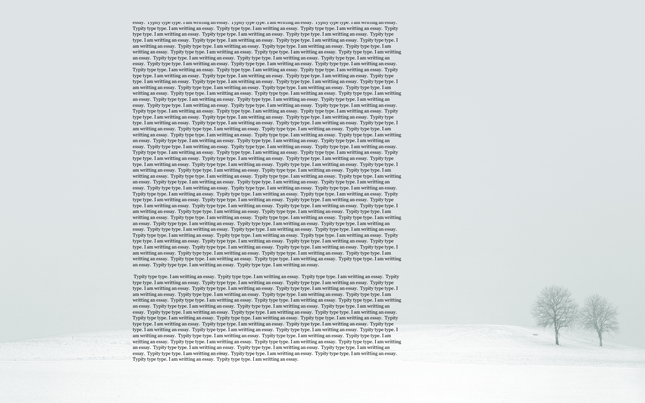
\includegraphics[width=130mm]{images/ommwriter2.png}
   \caption{...}
\end{figure}

Probably the biggest complaint comes from the limited number of themes. I was looking for a high contrast option, such as light green on a black field. There was nothing similar to this, and most themes were very low contrast and hard to read.

\begin{figure}
   \centering
      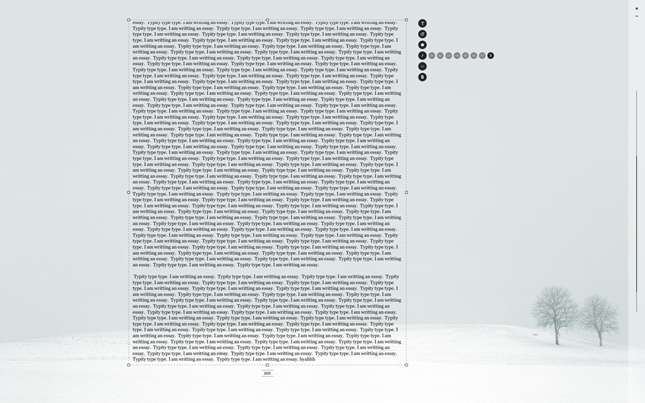
\includegraphics[width=130mm]{images/ommwriter3.png}
   \caption{...}
\end{figure}

The workspace was adjustable in size, and the user interface came and went based on mouse movement and typing speed, which was a nice touch. OmmWriter seemed the most polished of everything I tried out, and was the program I probably tried the hardest to emulate.

\section{coffee\_shop}

Screen shots of the program.

Talk a little about the development process. We talk about how features were implemented below, so just give an overview of what the program does.

\section{Evaluation of coffee\_shop}

\subsection{Development decisions}

I made some decisions while developing and designing coffee\_shop, which may be considered controversial or unintelligent. The two big decisions I made were to use Ruby as my programming language and Qt as my graphics framework.

\subsubsection{Ruby}

Ruby is an interesting beast. I selected it because I had little experience with the language and it had a very large community online. Since starting the project I have learned a lot about the language.

Ruby is a really fun language to write in, but it is not made to develop systems whose state changes during its run. Ruby works far better as a shell script or responder for a website because it can execute in entirety and doesn't need to jump around to a ton of objects already allocated. It's possible that a graphics framework could solve this, but I was unable to find one that did.

\subsubsection{Qt}

Qt is incredibly powerful, and RubyQt \cite{rubyqt} is probably the best UI toolkit available for Ruby. But Qt is written for Java and C++. Qt expects to have references to everything, and wants everything to be passed by reference. Ruby doesn't really work this way and because of it, hindered Qt's power.

Interestingly enough, a lot of the things I saw other applications doing that I thought were cool, were actually areas where people were hacking directly on the Qt source, or rewriting entire sections of the library. \cite{kwrite}.

In hindsight, if I were to use Qt, I would use it with C++, instead of one of it's many ports to other languages.

\subsection{Features and their implementations}

\subsubsection{File writing}

Pretty simple, although lots of discussion.

\subsubsection{Pagination}

The bane of my existence.

\subsubsection{Printing}

This was surprisingly easy thanks to Qt. All I really had to do was open a ``Qt::PrintDialog'', which prompted the user to select a printer, and then send a block of text to the object representation of the printer they selected.

\subsubsection{Customization and preference storing}

Storing customizations was a pretty easy technical challenge. It required creating a singleton class, which let me store key value pairs to it. Then we would write out the changes to disk on occasion. We would also make sure all of the data got written out when the program exited.

The biggest problem was trying to support configuration changes while the program was running. Often Qt objects didn't want to be redrawn. Unlike an element in the DOM tree which can be styled dynamically with ease, Qt often made strange choices when to redraw with the new settings it was given. It seems like these redrawing actions are a common problem in the Qt world. When I asked around Nokia and Qt's forums, I was told I should just modify the core Qt code to get the desirable effect I was looking for.

\section{Future Work}

I think there is lots of work to be done here, but I would argue against it. Instead of continuing to develop this application, I would recommend looking into building a web application that simulates the same experience. CSS makes it easier to iterate quickly on the design and layout, plus you can use the HTML5 local storage API to let the user work offline.

If you were to continue working on this project, I would focus on making the application easier to deploy across a wide variety of operating systems. I would also try and find a layout that works well on all screen sizes.

\section{Conclusion}

Overall, I am proud of the work I did, but in the future I would probably just make this on the web.

\newpage
\nocite{*}
\bibliographystyle{IEEEannot}
\bibliography{texreport}
\end{document}
